\documentclass[10pt]{article}         %% What type of document you're writing.

%%%%% Preamble

%% Packages to use

\usepackage{amsmath,amsfonts,amssymb}   %% AMS mathematics macros
\usepackage{graphicx}
\usepackage{lmodern}  % for bold teletype font
\usepackage{amsmath}  % for \hookrightarrow
\usepackage{xcolor}   % for \textcolor
\usepackage{listings}
\lstset{
  basicstyle=\ttfamily,
  columns=fullflexible,
  frame=single,
  breaklines=true,
  postbreak=\mbox{\textcolor{red}{$\hookrightarrow$}\space},
}

%% Title Information.

\title{HomeWork 04}
\author{Deep Dand}
%% \date{2 July 2004}           %% By default, LaTeX uses the current date

%%%%% The Document

\begin{document}

\maketitle

\begin{abstract}
KNN Regressor
\end{abstract}

\section{Problem 1}
\subsection{a}
You will modify the python code below to generate 1000 data points.
\\The code below generates 1000 data points. 

Code Begins
\lstinputlisting{hw4a.py}
Code ends

In the code, I have introduced a variable N to change the number of data points to be generated which will further be used to perform regression. 
\\Output\\
\begin{center}
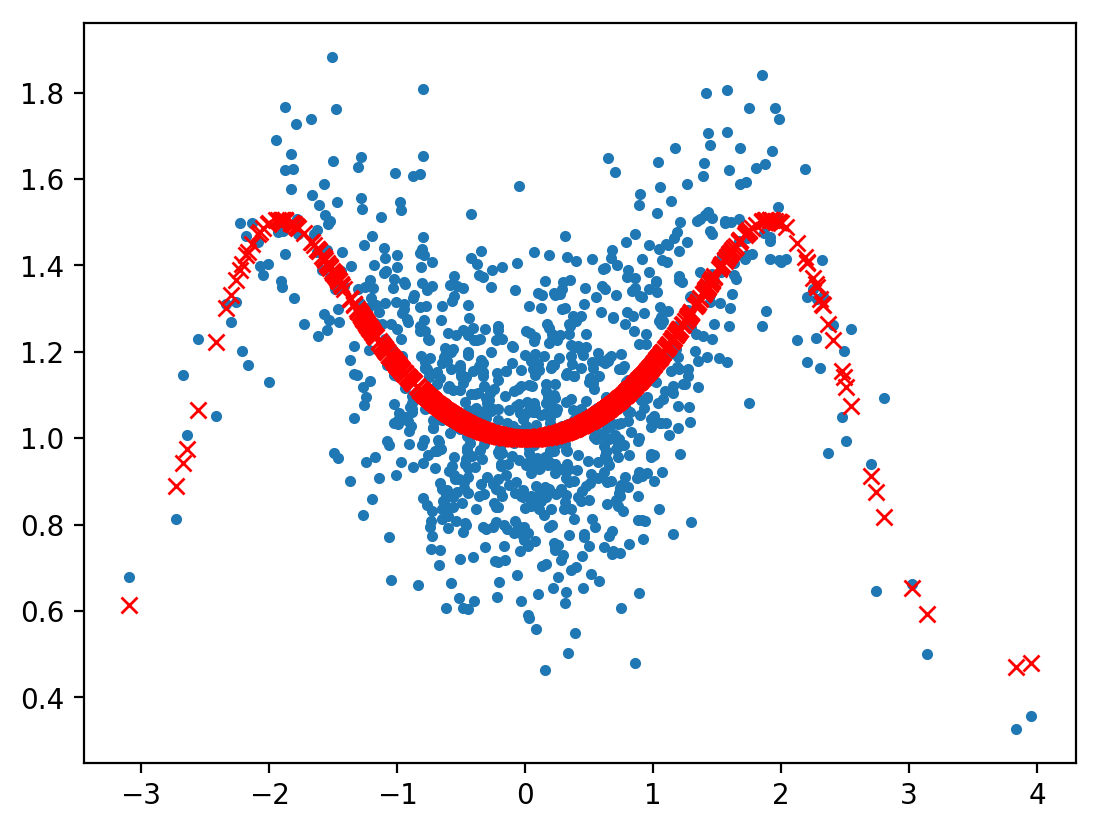
\includegraphics[scale=0.45]{HW4_PartA.png}
\end{center}
The chart above shows the distribution of the data points x and y across the plane.


\subsection{b,c}
Using 10-fold CV, you will report the three best values of k-neighbors that yield the best CV
Eout. You will vary the values of k in the following range: $$k = 2 * ((N+1)/2) - 1$$

You will report the best CV Eout.
Code Begins
\lstinputlisting{hw4btt.py}
Code ends. 
\\Output\\
\begin{center}
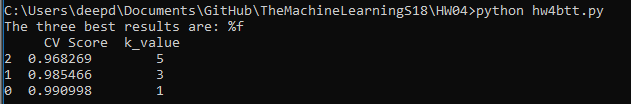
\includegraphics[scale=0.6]{hw4q1partc.png}
\end{center}
The code above has 2 parts to have odd values of "k" for number of neighbors.
In part 1, we divide the data in train and test so as to calculate the cross validation on test data in part 2. 

The main reason for doing so is, while the other for loop varies the value of k as,
$$k = 2 * ((N+1)/2) - 1$$
The Knn-regressor function gives error for indexes because it divides the data in test and train if not done explicitly and that doesn't match with the index that for loo tries to use. 

At the end, we display the three best results of cross validation and its corresponding "k" value which answers part C of the question as well.

\section{Problem 2}
Here is my attempt to iterate the code 100 times and save results. Somehow, the data-frame is getting over-written and so I am unable to store and generate histogram of the same. 
The code looks like, 
\lstinputlisting{hw4q2.py}

\end{document}

